\documentclass[12pt]{article}

\usepackage{graphicx}
\usepackage{caption}
\usepackage{subcaption}
\usepackage[spanish]{babel}
\usepackage[utf8]{inputenx}
\usepackage{anysize} 
\usepackage{amsmath}
\usepackage{listings}
%\usepackage{wrapfig} % paquete gráfico... quizás es necesario actualizar paquetes en kile
\usepackage{hyperref}

\usepackage{fancyhdr}
\pagestyle{fancy}

\hypersetup{
    colorlinks,%
    citecolor=black,%
    filecolor=black,%
    linkcolor=black,%
    urlcolor=black
}
\marginsize{2cm}{2cm}{1cm}{1cm} %izq der arriva abajo

\title{Informe preliminar}
\author{Facundo Nahuel Uriel Silva}

\lhead{ \chaptername }

 
\begin{document}

  %Caratula
  \newpage
  \thispagestyle{empty}
  
  \begin{center}
    
\includegraphics[width=250px]{../logo_fiuba_alta.jpg} 

  \vspace{40px}

   {\bf \Large{Trabajo Profesional de Ingeniería Electrónica} }
  
  \vspace{30px}

  \huge{Sistema de control para proceso de sinterizado de nano estructuras }
  
  \vspace{40px}
  
  \huge{\textit{Especificaciones Técnicas} }
  
  \vspace{30px}
  \Large{ V1.2 }

  \end{center}

\vspace{100px}

   \begin{bf}
    \begin{Large}
      \begin{tabbing}
	\= ----- \= ----- \= --------------------- \= \kill
	\> Integrantes:\\
	\\
	  \>\> Estanislao López Morgan \\
	  \>\>\>  Padrón:	\> 84546 \\
	  \>\>\>  Mail:	\>\url{estanux@gmail.com} \\
	\\
	  \>\> Facundo Nahuel Uriel Silva\\
	  \>\>\>  Padrón:	\> 86881 \\
	  \>\>\>  Mail:	\> \url{fanaur@gmail.com}\\
      \end{tabbing}
    \end{Large}
  \end{bf}

\newpage
\thispagestyle{empty}
\vspace{80px}

\begin{large}
     \begin{bf} 
         Historial
      \end{bf}
\end{large}

\vspace{20px}

%------tabla historial----
  \vspace{3px}
  \begin{tabular}{|p{50px}|p{40px}|p{165px}|p{120px}|}
   \hline
      \textbf{Fecha}       &   
      \textbf{Versión}     &   
      \textbf{Descripción} & 
      \textbf{Autores}      \\
    \hline
      \multicolumn{1}{|p{50px}|}{ 
	%\textbf{ } \newline \vspace{5px}  % Tema
	28/08/12
     }&
    
      \multicolumn{1}{|p{40px}|}{
	 %\begin{center}
	 \hspace{12px}
           1.0
	  %\end{center}
     }&
     
       \multicolumn{1}{ |p{165px}| }{
	Especificaciones Técnicas			 
      }&
      
     \multicolumn{1}{|p{120px}|}{ 
      Silva - López Morgan
     } \\
     \hline
    
    \multicolumn{1}{|p{50px}|}{ 
	%\textbf{ } \newline \vspace{5px}  % Tema
	06/09/12
     }&
    
      \multicolumn{1}{|p{40px}|}{
	 %\begin{center}
	 \hspace{12px}
           1.1
	  %\end{center}
     }&
     
       \multicolumn{1}{ |p{165px}| }{
	Se especifican las interfases para el conexionado de los sensores.
      }&
      
     \multicolumn{1}{|p{120px}|}{ 
      Silva - López Morgan
     } \\
     \hline
    
    \multicolumn{1}{|p{50px}|}{ 
	%\textbf{ } \newline \vspace{5px}  % Tema
	06/09/12
     }&
    
      \multicolumn{1}{|p{40px}|}{
	 %\begin{center}
	 \hspace{12px}
           1.2
	  %\end{center}
     }&
     
       \multicolumn{1}{ |p{165px}| }{
	Corrección de la posición de un sensor de tensión en el diagrama en bloques.
      }&
      
     \multicolumn{1}{|p{120px}|}{ 
      Silva - López Morgan
     } \\
     \hline

\end{tabular}
  %------end tabla-----

  %Indice de contenidos
  \newpage
  
  \thispagestyle{empty} \tableofcontents \thispagestyle{empty} %asi se sace el numero de pagina

  %Comienzo
  \newpage
  \setcounter{page}{1}

  %%%%%%%%%%%%%%%%%%%%%%%%%%%%%%%%%%%%%%%%%%%%%%%%%%%%%%%%%%%%%%%%%%%%%%%%%%%%%%%%%%%%%%%%%%%%%%%%%%%%%%%%%%%%%%%%%%%%%%%%%%%%%%%%%%%%%%%%%%%%%%%%%%%%%
  %%%%%%%%%%%%%%%%%%%%%%%%%%%%%%%%%%%%%%%%%%%%%%%%%%%%%%%%%%%%%%%%%%%%%%%%%%%%%%%%%%%%%%%%%%%%%%%%%%%%%%%%%%%%%%%%%%%%%%%%%%%%%%%%%%%%%%%%%%%%%%%%%%%%%
  
  \section{Especificaciones de hardware}

    \subsection{Aspectos eléctricos}
      \begin{itemize}
	\item Tensión alimentación: 220VAC/50Hz.
	\item Consumo máximo: 1A.$*^{1}$
	\item Pico de corriente de sinterizado máximo: 1KA. $*^{2}$
	\item Impedancia máxima de la muestra: 1$\Omega$. 
	\end{itemize}
     
    \begin{tabbing}
      \= ----- \= ----- \= --------------------- \= \kill
      \> $*^{1}$:\>	El consumo máximo estará fijado por la fuente que se utilice y esta por el transformador. \\
      \> $*^{2}$:\>	La corriente máxima de pico de sinterizado puede ser incrementada hasta 10 kA si se amplía\\
         	\>\>	el banco de capacitores, se remplaza los contactores y el cableado correspondiente.\\
     \end{tabbing}

    \subsection{Almacenamientos de datos}
      
      \begin{itemize}
	\item Memoria flash en soporte SD Card.
	\item Memoria flash en soporte pendrive USB 2.0.
      \end{itemize}

    \subsection{Comunicación}
      
      \begin{itemize}
	\item Comunicación USB 2.0 con la PC. $*^{3}$
      \end{itemize}
    
      \begin{tabbing}
	\= ----- \= ----- \= --------------------- \= \kill
	\>$*^{3}$: \>Se utiliza un bridge RS232-USB interno. \\
       \end{tabbing}
	
    \subsection{Periféricos del dispositivo}
      \begin{itemize}
	\item Display gráfico de 128x64 pixels.
	\item Teclado de 4 teclas.
	\item Sensor de corriente.
	\item Sensores de tensión $\times$ 3.
	\item Sensor de temperatura.
      \end{itemize}

    \subsection{Interfases del dispositivo}
      \begin{itemize}
	\item Entrada de 0-5V $\times$ 3.$*^{4}*^{5}$
	\item Entrada de 5-20mA $\times$ 1.$*^{4}$
	\item Puertos UART $\times$ 3.$*^{6}$
	\item Bus $ I^{2}C $.$*^{6}$
      \end{itemize}

      \begin{tabbing}
       \= ----- \= ----- \= --------------------- \= \kill
	\> $*^{4}$: \>Interfases configurables desde el programa de PC. \\
	\> $*^{5}$: \>Interfases usadas para los sensores de tensión y corriente \\
	\> $*^{6}$: \>Interfases reservadas para usos futuros. \\
      \end{tabbing}

    \subsection{Seguridad}
      \begin{itemize}
	\item Descarga segura del banco de capacitores.
	\item Sirena sonora.
	\item Luces de señalización $\times$ 3.
	\item Banco de capacitores ubicados dentro del gabinete del dispositivo .
	\item Revestimiento eléctricamente aislante del gabinete del dispositivo.
	\item Protección contra corto circuito.
	\item Botón de parada de emergencia.
      \end{itemize}

    \subsection{Aspectos mecánicos}
      \begin{itemize}
	\item No se brinda la función de prensado de la muestra. $*^{7}$
	\item Gabinete con 4 ruedas. 
	\item No se brinda el recipiente contenedor de la muestra de polvo.
      \end{itemize}

      \begin{tabbing}
       \= ----- \= ----- \= --------------------- \= \kill
	\> $*^{7}$: \>  La muestra debe estar prensada previamente al momento de realizar el \\
	    \>\>	proceso sinterizado.\\
      \end{tabbing}

    \subsection{Aspectos de operativos}
      \begin{itemize}
	\item Uso máximo mensual: 60 veces. $*^{8}$
      \end{itemize}
    
      \begin{tabbing}
	\= ----- \= ----- \= --------------------- \= \kill
	\> $*^{8}$: \>Se estima un promedio de 2 usos diarios. \\
      \end{tabbing}

\newpage

    \subsection{ Croquis }

    \begin{figure}[h!]
    \centering
    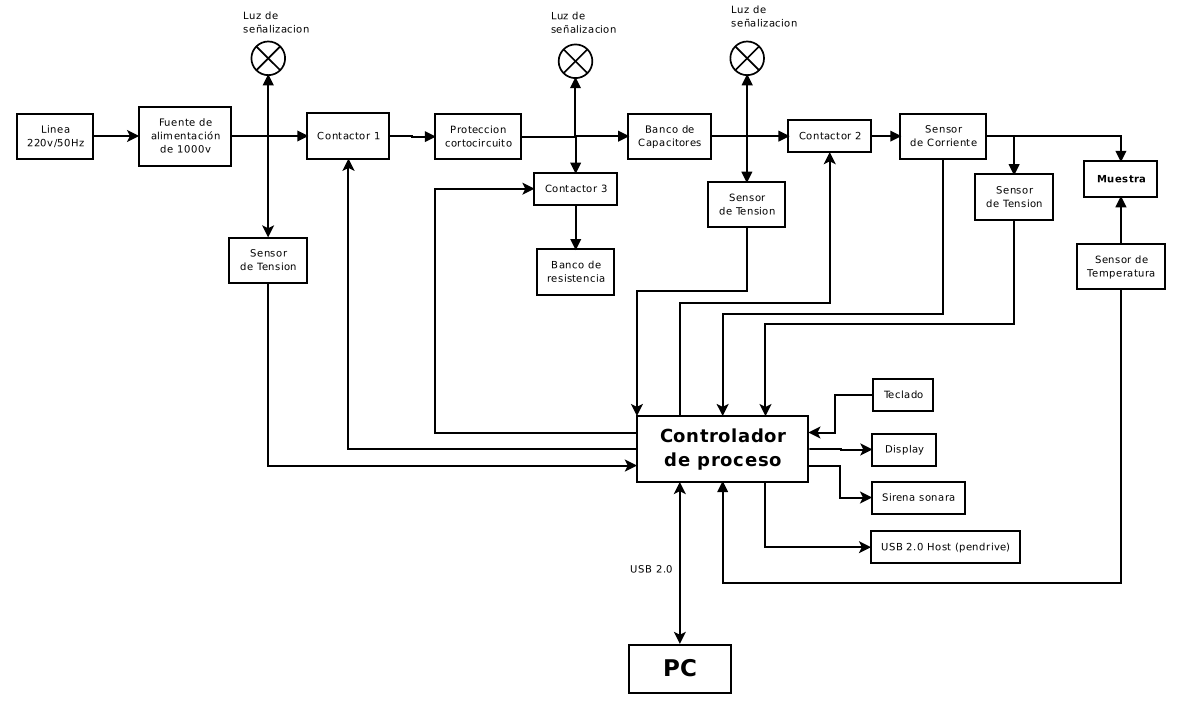
\includegraphics[width=500px]{../../Documentacion/Diagramas/diagramaBloquesEspecificaciones.png}
    % diagramaBloquesEspecificaciones.png: 1170x708 pixel, 96dpi, 30.95x18.73 cm, bb=0 0 877 531
    \caption{Interconeccion entre los bloques del sistema}
    \end{figure}

  %%%%%%%%%%%%%%%%%%%%%%%%%%%%%%%%%%%%%%%%%%%%%%%%%%%%%%%%%%%%%%%%%%%%%%%%%%%%%%%%%%%%%%%%%%%%%%%%%%%%%%%%%%%%%%%%%%%%%%%%%%%%%%%%%%%%%%%%%%%%%%%%%%%%%
  %%%%%%%%%%%%%%%%%%%%%%%%%%%%%%%%%%%%%%%%%%%%%%%%%%%%%%%%%%%%%%%%%%%%%%%%%%%%%%%%%%%%%%%%%%%%%%%%%%%%%%%%%%%%%%%%%%%%%%%%%%%%%%%%%%%%%%%%%%%%%%%%%%%%%
\newpage

  \section{Especificaciones de software}

    El control, administración, monitoreo y recolección de datos del dispositivo de control del proceso de sinterizado se harán a través de 
    un programa de PC con las siguiente características:
    
    \begin{itemize}
      \item Plataforma Windows XP/7 y GNU Linux.
      \item Formato de datos exportados CSV.
      \item Control de acceso.
      \item Base de datos.
    \end{itemize}
  
    \subsection{Pantallas}
      El programa contara con las siguientes pantallas:

    \begin{itemize}
      \item Login.      
      \item ABM usuarios.
      \item Monitoreo dispositivo.
      \item Parametrización del experimento.
      \item Control experimentación.
      \item Descarga de datos del experimento.
      \item Exportación de resultados de experimentación.
      \item Ploteo de resultados del experimento.
    \end{itemize}
  

%   %Bibliografia
%   \newpage
% 
%   \begin{thebibliography}{1}
%     \bibitem{} 
% 
%   \end{thebibliography}
    

\end{document}
